%!Tex Root = ../Tutorat5.tex
% ./Packete.tex
% ./Design.tex
% ./Deklarationen.tex
% ./Aufgabe1.tex
% ./Aufgabe3.tex
% ./Bonus.tex

\section{Task 2}

\setcounter{task}{1}

\begin{frame}[allowframebreaks]{Task 2}{}
  \begin{tasknoinc}
    \centering
    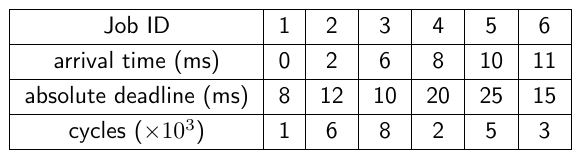
\includegraphics[width=0.8\paperheight]{./figures/task2.png}
  \end{tasknoinc}
  \begin{requirements}
    \begin{itemize}
      \item $V^{\prime}\left(\left[z, z^{\prime}\right]\right)=\left\{v_i \in V: z \leq a_i<d_i \leq z^{\prime}\right\}$
      \item $G\left(\left[z, z^{\prime}\right]\right)=\sum_{v_i \in V^{\prime}\left(\left[z, z^{\prime}\right]\right)} c_i /\left(z^{\prime}-z\right)$
    \end{itemize}
  \end{requirements}
\end{frame}

\begin{frame}[allowframebreaks]{Task 2}{}
  \begin{solutionnoinc}
    \begin{ganttchart}[
        x unit=0.4cm,
        y unit chart=0.7cm,
        canvas/.style={draw=none,fill=none}, % remove canvas borders, etc
        vgrid={*1{draw=black!12}},           % vertical gray lines every unit
        inline,                              % draw bars inline
        group/.style={draw=none,fill=none},  % remove group borders, etc
        bar top shift=0.1,                   % give bar 10% padding top/bottom
        bar height=0.8,                      % bar size 80% of vertical space
        y unit title=0.5cm,                  % crop titles a little smaller
        title/.style={draw=none,fill=none},  % remove title borders, etc
        include title in canvas=false        % no vertical grid in title
      ]{-1}{26}

      \gantttitle{0}{2}
      \gantttitle{2}{2}
      \gantttitle{4}{2}
      \gantttitle{6}{2}
      \gantttitle{8}{2}
      \gantttitle{10}{2}
      \gantttitle{12}{2}
      \gantttitle{14}{2}
      \gantttitle{16}{2}
      \gantttitle{18}{2}
      \gantttitle{20}{2}
      \gantttitle{22}{2}
      \gantttitle{24}{2}
      \gantttitle{26}{2} \\

      \ganttgroup[inline=false]{$T_{1}$}{0}{1}
      \ganttbar[bar/.style={fill=red, fill opacity=0.3}]{1 (n=1)}{0}{7}\\

      \ganttgroup[inline=false]{$T_{2}$}{0}{1}
      \ganttbar[bar/.style={fill=orange, fill opacity=0.3}]{2 (n=6)}{2}{11}\\

      \ganttgroup[inline=false]{$T_{3}$}{0}{1}
      \ganttbar[bar/.style={fill=yellow, fill opacity=0.3}]{3 (n=8)}{6}{9}\\

      \ganttgroup[inline=false]{$T_{4}$}{0}{1}
      \ganttbar[bar/.style={fill=green, fill opacity=0.3}]{4 (n=2)}{8}{19}\\

      \ganttgroup[inline=false]{$T_{5}$}{0}{1}
      \ganttbar[bar/.style={fill=blue, fill opacity=0.3}]{5 (n=5)}{10}{24}\\

      \ganttgroup[inline=false]{$T_{6}$}{0}{1}
      \ganttbar[bar/.style={fill=cyan, fill opacity=0.3}]{6 (n=3)}{11}{14}

    \end{ganttchart}
  \end{solutionnoinc}
  \begin{solutionnoinc}
    \tiny
    \begin{columns}
      \begin{column}{0.33\textwidth}
        \begin{itemize}
          \item $G([0, 8]) = \frac{1}{8} = 0.125$
          \item $G([0, 12]) = \frac{1+6+8}{12} = 1.25$
          \item $G([0, 10]) = \frac{1+8}{10} = 0.9$
          \item $G([0, 20]) = \frac{1+6+8+2+3}{20} = 1$
          \item $G([0, 25]) = \frac{1+6+8+2+3+5}{25} = 1$
          \item $G([0, 15]) = \frac{1+6+8+3}{15} = 1.2$
          \item $G([2, 12]) = \frac{6+8}{10} = 1.4$
        \end{itemize}
      \end{column}
      \begin{column}{0.33\textwidth}
        \begin{itemize}
          \item $G([2, 10]) = \frac{8}{8} = 1$
          \item $G([2, 20]) = \frac{6+8+2+3}{18} = 1.06$
          \item $G([2, 25]) = \frac{6+8+2+3+5}{23} = 1.04$
          \item $G([2, 15]) = \frac{6+8+3}{13} = 1.31$
          \item $\boxed{G([6, 10]) = \frac{8}{4} = 2}$
          \item $G([6, 20]) = \frac{8+2+3}{14} = 0.93$
          \item $G([6, 25]) = \frac{8+2+3+5}{19} = 0.95$
        \end{itemize}
      \end{column}
      \begin{column}{0.33\textwidth}
        \begin{itemize}
          \item $G([6, 15]) = \frac{8+3}{9} = 1.22$
          \item $G([8, 20]) = \frac{2+3}{12} = 0.42$
          \item $G([8, 25]) = \frac{2+3+5}{17} = 0.59$
          \item $G([8, 15]) = \frac{3}{7} = 0.43$
          \item $G([10, 25]) = \frac{5+3}{15} = 5.3$
          \item $G([10, 15]) = \frac{3}{5} = 0.6$
          \item $G([11, 15]) = \frac{3}{4} = 0.75$
        \end{itemize}
      \end{column}
    \end{columns}
  \end{solutionnoinc}
  \begin{solutionnoinc}
    \begin{ganttchart}[
        x unit=0.4cm,
        y unit chart=0.7cm,
        canvas/.style={draw=none,fill=none}, % remove canvas borders, etc
        vgrid={*1{draw=black!12}},           % vertical gray lines every unit
        inline,                              % draw bars inline
        group/.style={draw=none,fill=none},  % remove group borders, etc
        bar top shift=0.1,                   % give bar 10% padding top/bottom
        bar height=0.8,                      % bar size 80% of vertical space
        y unit title=0.5cm,                  % crop titles a little smaller
        title/.style={draw=none,fill=none},  % remove title borders, etc
        include title in canvas=false        % no vertical grid in title
      ]{-1}{22}

      \gantttitle{0}{2}
      \gantttitle{2}{2}
      \gantttitle{4}{2}
      \gantttitle{6}{2}
      \gantttitle{8}{2}
      \gantttitle{10}{2}
      \gantttitle{12}{2}
      \gantttitle{14}{2}
      \gantttitle{16}{2}
      \gantttitle{18}{2}
      \gantttitle{20}{2}
      \gantttitle{22}{2} \\

      \ganttgroup[inline=false]{$T_{1}$}{0}{1}
      \ganttbar[bar/.style={fill=red, fill opacity=0.3}]{1 (n=1)}{0}{5}\\

      \ganttgroup[inline=false]{$T_{2}$}{0}{1}
      \ganttbar[bar/.style={fill=orange, fill opacity=0.3}]{2 (n=6)}{2}{7}\\

      \ganttgroup[inline=false]{$T_{4}$}{0}{1}
      \ganttbar[bar/.style={fill=green, fill opacity=0.3}]{4 (n=2)}{6}{15}\\

      \ganttgroup[inline=false]{$T_{5}$}{0}{1}
      \ganttbar[bar/.style={fill=blue, fill opacity=0.3}]{5 (n=5)}{6}{20}\\

      \ganttgroup[inline=false]{$T_{6}$}{0}{1}
      \ganttbar[bar/.style={fill=cyan, fill opacity=0.3}]{6 (n=3)}{7}{10}
    \end{ganttchart}
  \end{solutionnoinc}
  \begin{solutionnoinc}
    \scriptsize
    \begin{columns}
      \begin{column}[t]{0.5\textwidth}
        \begin{itemize}
          \item $G([0, 6]) = \frac{1}{6} = 0.17$
          \item $G([0, 8]) = \frac{1+6}{8} = 0.875$
          \item $G([0, 16]) = \frac{1+6+2+3}{16} = 0.75$
          \item $G([0, 21]) = \frac{1+6+2+5+3}{21} = 0.81$
          \item $G([0, 11]) = \frac{1+6+3}{11} = 0.91$
          \item $G([2, 8]) = \frac{6}{6} = 1$
          \item $G([2, 16]) = \frac{6+2+3}{14} = 0.79$
          \item $G([2, 21]) = \frac{6+2+5+3}{19} = 0.84$
        \end{itemize}
      \end{column}
      \begin{column}[t]{0.5\textwidth}
        \begin{itemize}
          \item $\boxed{G([2, 11]) = \frac{6+3}{9} = 1}$
          \item $G([6, 16]) = \frac{2+3}{10} = 0.5$
          \item $G([6, 21]) = \frac{2+5+3}{15} = 0.67$
          \item $G([6, 11]) = \frac{3}{5} = 0.6$
          \item $G([7, 11]) = \frac{3}{4} = 0.75$
        \end{itemize}
      \end{column}
    \end{columns}
  \end{solutionnoinc}
  \begin{solutionnoinc}
    \begin{ganttchart}[
        x unit=0.4cm,
        y unit chart=0.7cm,
        canvas/.style={draw=none,fill=none}, % remove canvas borders, etc
        vgrid={*1{draw=black!12}},           % vertical gray lines every unit
        inline,                              % draw bars inline
        group/.style={draw=none,fill=none},  % remove group borders, etc
        bar top shift=0.1,                   % give bar 10% padding top/bottom
        bar height=0.8,                      % bar size 80% of vertical space
        y unit title=0.5cm,                  % crop titles a little smaller
        title/.style={draw=none,fill=none},  % remove title borders, etc
        include title in canvas=false        % no vertical grid in title
      ]{-1}{12}

      \gantttitle{0}{2}
      \gantttitle{2}{2}
      \gantttitle{4}{2}
      \gantttitle{6}{2}
      \gantttitle{8}{2}
      \gantttitle{10}{2}
      \gantttitle{12}{2} \\

      \ganttgroup[inline=false]{$T_{1}$}{0}{1}
      \ganttbar[bar/.style={fill=red, fill opacity=0.3}]{1 (n=1)}{0}{1}\\

      \ganttgroup[inline=false]{$T_{4}$}{0}{1}
      \ganttbar[bar/.style={fill=green, fill opacity=0.3}]{4 (n=2)}{2}{6}\\

      \ganttgroup[inline=false]{$T_{5}$}{0}{1}
      \ganttbar[bar/.style={fill=blue, fill opacity=0.3}]{5 (n=5)}{2}{11}\\
    \end{ganttchart}
  \end{solutionnoinc}
  \begin{solutionnoinc}
    \begin{itemize}
      \item $G([0, 2]) = \frac{1}{2} = 0.5$
      \item $G([0, 7]) = \frac{1+2}{7} = 0.43$
      \item $G([0, 12]) = \frac{1+2+5}{12} = 0.67$
      \item $G([2, 7]) = \frac{2}{5} = 0.4$
      \item $\boxed{G([2, 12]) = \frac{2+5}{10} = 0.7}$
    \end{itemize}
  \end{solutionnoinc}
  \begin{solutionnoinc}
    \begin{ganttchart}[
        x unit=0.4cm,
        y unit chart=0.7cm,
        canvas/.style={draw=none,fill=none}, % remove canvas borders, etc
        vgrid={*1{draw=black!12}},           % vertical gray lines every unit
        inline,                              % draw bars inline
        group/.style={draw=none,fill=none},  % remove group borders, etc
        bar top shift=0.1,                   % give bar 10% padding top/bottom
        bar height=0.8,                      % bar size 80% of vertical space
        y unit title=0.5cm,                  % crop titles a little smaller
        title/.style={draw=none,fill=none},  % remove title borders, etc
        include title in canvas=false        % no vertical grid in title
      ]{-1}{2}

      \gantttitle{0}{2}
      \gantttitle{2}{2} \\

      \ganttgroup[inline=false]{$T_{1}$}{0}{1}
      \ganttbar[bar/.style={fill=red, fill opacity=0.3}]{1 (n=1)}{0}{1}\\
    \end{ganttchart}
  \begin{itemize}
    \item $\boxed{G([0, 2]) = \frac{1}{2} = 0.5}$
  \end{itemize}
  \end{solutionnoinc}
\end{frame}

\begin{frame}[allowframebreaks]{Task 2}{}
  \begin{solution}
    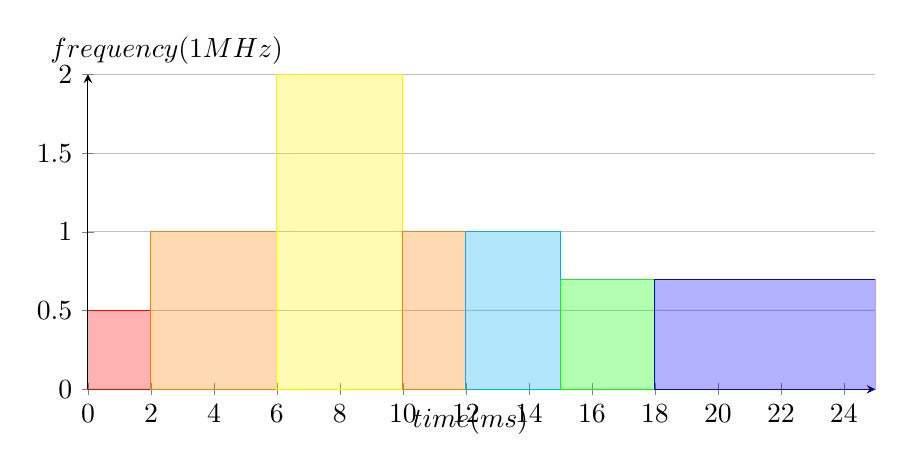
\begin{tikzpicture}
      \begin{axis}[x=0.4cm, y=2cm, xtick={0, 2, ..., 25}, ytick={0, 0.5, ...,2}, axis lines=left,
        ymajorgrids=true, ymin=0, xlabel=$time (ms)$, xlabel style={at={(0.4,-0.1)}, anchor=west},
        ylabel=$frequency (1 MHz)$, ylabel style={rotate=-90,at={(0.1,1)}, anchor=south}
        ]
      \addplot [
        ybar interval,
        xtick=data,
        x tick label style={
        rotate=90,
        anchor=east,
        },
        color=red, fill=red, fill opacity=0.3
      ] coordinates {
        (0,0.5) (2,0.5)
      };
      \addplot [
        ybar interval,
        xtick=data,
        x tick label style={
        rotate=90,
        anchor=east,
        },
        color=orange, fill=orange, fill opacity=0.3
      ] coordinates {
        (2,1) (6,1)
      };
      \addplot [
        ybar interval,
        xtick=data,
        x tick label style={
        rotate=90,
        anchor=east,
        },
        color=yellow, fill=yellow, fill opacity=0.3
      ] coordinates {
        (6,2) (10,2)
      };
      \addplot [
        ybar interval,
        xtick=data,
        x tick label style={
        rotate=90,
        anchor=east,
        },
        color=orange, fill=orange, fill opacity=0.3
      ] coordinates {
        (10,1) (12,1)
      };
      \addplot [
        ybar interval,
        xtick=data,
        x tick label style={
        rotate=90,
        anchor=east,
        },
        color=cyan, fill=cyan, fill opacity=0.3
      ] coordinates {
        (12,1) (15,1)
      };
      \addplot [
        ybar interval,
        xtick=data,
        x tick label style={
        rotate=90,
        anchor=east,
        },
        color=green, fill=green, fill opacity=0.3
      ] coordinates {
        (15,0.7) (18,.07)
      };
      \addplot [
        ybar interval,
        xtick=data,
        x tick label style={
        rotate=90,
        anchor=east,
        },
        color=blue, fill=blue, fill opacity=0.3
      ] coordinates {
        (18,0.7) (25,0.7)
      };
    \end{axis}
    \end{tikzpicture}
  \end{solution}
\end{frame}

\begin{frame}[allowframebreaks]{Task 2}{}
  \begin{solutionnoinc}
    \begin{ganttchart}[
        x unit=0.4cm,
        y unit chart=0.7cm,
        canvas/.style={draw=none,fill=none}, % remove canvas borders, etc
        vgrid={*1{draw=black!12}},           % vertical gray lines every unit
        inline,                              % draw bars inline
        group/.style={draw=none,fill=none},  % remove group borders, etc
        bar top shift=0.1,                   % give bar 10% padding top/bottom
        bar height=0.8,                      % bar size 80% of vertical space
        y unit title=0.5cm,                  % crop titles a little smaller
        title/.style={draw=none,fill=none},  % remove title borders, etc
        include title in canvas=false        % no vertical grid in title
      ]{-1}{26}

      \gantttitle{0}{2}
      \gantttitle{2}{2}
      \gantttitle{4}{2}
      \gantttitle{6}{2}
      \gantttitle{8}{2}
      \gantttitle{10}{2}
      \gantttitle{12}{2}
      \gantttitle{14}{2}
      \gantttitle{16}{2}
      \gantttitle{18}{2}
      \gantttitle{20}{2}
      \gantttitle{22}{2}
      \gantttitle{24}{2}
      \gantttitle{26}{2} \\

      \ganttgroup[inline=false]{$T_{1}$}{0}{1}
      \ganttbar[bar/.style={fill=red, fill opacity=0.3}]{1 (n=1)}{0}{7}\\

      \ganttgroup[inline=false]{$T_{2}$}{0}{1}
      \ganttbar[bar/.style={fill=orange, fill opacity=0.3}]{2 (n=6)}{2}{11}\\

      \ganttgroup[inline=false]{$T_{3}$}{0}{1}
      \ganttbar[bar/.style={fill=yellow, fill opacity=0.3}]{3 (n=8)}{6}{9}\\

      \ganttgroup[inline=false]{$T_{4}$}{0}{1}
      \ganttbar[bar/.style={fill=green, fill opacity=0.3}]{4 (n=2)}{8}{19}\\

      \ganttgroup[inline=false]{$T_{5}$}{0}{1}
      \ganttbar[bar/.style={fill=blue, fill opacity=0.3}]{5 (n=5)}{10}{24}\\

      \ganttgroup[inline=false]{$T_{6}$}{0}{1}
      \ganttbar[bar/.style={fill=cyan, fill opacity=0.3}]{6 (n=3)}{11}{14}
    \end{ganttchart}
  \end{solutionnoinc}
  \begin{solutionnoinc}
    \begin{itemize}
      \item $\boxed{G([0, 8]) = \frac{1}{8} = 0.125}$
    \end{itemize}
  \end{solutionnoinc}
  \framebreak
  \begin{solutionnoinc}
    \begin{ganttchart}[
        x unit=0.4cm,
        y unit chart=0.7cm,
        canvas/.style={draw=none,fill=none}, % remove canvas borders, etc
        vgrid={*1{draw=black!12}},           % vertical gray lines every unit
        inline,                              % draw bars inline
        group/.style={draw=none,fill=none},  % remove group borders, etc
        bar top shift=0.1,                   % give bar 10% padding top/bottom
        bar height=0.8,                      % bar size 80% of vertical space
        y unit title=0.5cm,                  % crop titles a little smaller
        title/.style={draw=none,fill=none},  % remove title borders, etc
        include title in canvas=false        % no vertical grid in title
      ]{-1}{8}

      \gantttitle{0}{2}
      \gantttitle{2}{2}
      \gantttitle{4}{2}
      \gantttitle{6}{2}
      \gantttitle{8}{2}
      \gantttitle{10}{2}
      \gantttitle{12}{2}
      \gantttitle{14}{2}
      \gantttitle{16}{2}
      \gantttitle{18}{2}
      \gantttitle{20}{2} \\

      \ganttgroup[inline=false]{$T_{1}$}{0}{1}
      \ganttbar[bar/.style={fill=red, fill opacity=0.3}]{1 (n=0.75)}{2}{7}\\

      \ganttgroup[inline=false]{$T_{2}$}{0}{1}
      \ganttbar[bar/.style={fill=orange, fill opacity=0.3}]{2 (n=6)}{2}{11}\\
    \end{ganttchart}
  \end{solutionnoinc}
  \framebreak
  \begin{solutionnoinc}
    \begin{itemize}
      \item $G([2, 8]) = \frac{1-0.125\cdot 2}{6} = 0.125$
      \item $\boxed{G([2, 12]) = \frac{(1-0.125\cdot 2) + 6}{10} = 0.675}$
      \item $d_1 = 8 > 12 = d_2$, Task 1 has ealier dealine (EDF)
      \item $\displaystyle T_1 = \frac{0.75}{0.675} \approx 1.11, d_1^* = 2 + 1.11 = 3.11$
    \end{itemize}
  \end{solutionnoinc}
  \framebreak
  \begin{solutionnoinc}
    \begin{ganttchart}[
        x unit=0.4cm,
        y unit chart=0.7cm,
        canvas/.style={draw=none,fill=none}, % remove canvas borders, etc
        vgrid={*1{draw=black!12}},           % vertical gray lines every unit
        inline,                              % draw bars inline
        group/.style={draw=none,fill=none},  % remove group borders, etc
        bar top shift=0.1,                   % give bar 10% padding top/bottom
        bar height=0.8,                      % bar size 80% of vertical space
        y unit title=0.5cm,                  % crop titles a little smaller
        title/.style={draw=none,fill=none},  % remove title borders, etc
        include title in canvas=false        % no vertical grid in title
      ]{-1}{12}

      \gantttitle{0}{2}
      \gantttitle{2}{2}
      \gantttitle{4}{2}
      \gantttitle{6}{2}
      \gantttitle{8}{2}
      \gantttitle{10}{2}
      \gantttitle{12}{2} \\

      \ganttgroup[inline=false]{$T_{2}$}{0}{1}
      \ganttbar[bar/.style={fill=orange, fill opacity=0.3}]{2 (n=4.05)}{6}{11}\\

      \ganttgroup[inline=false]{$T_{3}$}{0}{1}
      \ganttbar[bar/.style={fill=yellow, fill opacity=0.3}]{3 (n=8)}{6}{9}\\
    \end{ganttchart}
  \end{solutionnoinc}
  \framebreak
  \begin{solutionnoinc}
    \begin{itemize}
      \item $G([6, 10]) = \frac{6 - (0.675 \cdot (4 - 1.111))}{4} = 1.01$
      \item $\boxed{G([6, 12]) = \frac{6 - (0.675 \cdot (4 - 1.111)) + 8}{6} = 2.01}$
      \item $d_2 = 12 > 10 = d_3$, Task 3 has ealier dealine (EDF)
      \item $T_3=\frac{8}{2.01} \approx 3.98, d_3^* = 6 + 3.98 \approx 10$
      % \item $T_2=\frac{4.05}{2.01} \approx 2.01, d_2^* = 6 + 2.01 \approx 10$
    \end{itemize}
  \end{solutionnoinc}
  \framebreak
  \begin{solutionnoinc}
    \begin{ganttchart}[
        x unit=0.4cm,
        y unit chart=0.7cm,
        canvas/.style={draw=none,fill=none}, % remove canvas borders, etc
        vgrid={*1{draw=black!12}},           % vertical gray lines every unit
        inline,                              % draw bars inline
        group/.style={draw=none,fill=none},  % remove group borders, etc
        bar top shift=0.1,                   % give bar 10% padding top/bottom
        bar height=0.8,                      % bar size 80% of vertical space
        y unit title=0.5cm,                  % crop titles a little smaller
        title/.style={draw=none,fill=none},  % remove title borders, etc
        include title in canvas=false        % no vertical grid in title
      ]{-1}{20}

      \gantttitle{0}{2}
      \gantttitle{2}{2}
      \gantttitle{4}{2}
      \gantttitle{6}{2}
      \gantttitle{8}{2}
      \gantttitle{10}{2}
      \gantttitle{12}{2}
      \gantttitle{14}{2}
      \gantttitle{16}{2}
      \gantttitle{18}{2}
      \gantttitle{20}{2}\\

      \ganttgroup[inline=false]{$T_{2+3}$}{0}{1}
      \ganttbar[bar/.style={fill=yellow, fill opacity=0.3}]{\qquad 2+3 (n=2.01)}{8}{9}
      \ganttbar[bar/.style={fill=orange, fill opacity=0.3}]{}{10}{11}\\

      \ganttgroup[inline=false]{$T_{4}$}{0}{1}
      \ganttbar[bar/.style={fill=green, fill opacity=0.3}]{4 (n=2)}{8}{19}\\
    \end{ganttchart}
  \end{solutionnoinc}
  \framebreak
  \begin{solutionnoinc}
    \begin{itemize}
      \item $G([8, 10]) = \frac{8-2.01 \cdot 2}{2} \approx 1.99$
      \item $\boxed{G([8, 12]) = \frac{6-0.675 \cdot (4-1.111) + 8-2.01 \cdot 2}{4} \approx 2.01}$
      \item $G([8, 20]) = \frac{6-0.675 \cdot (4-1.111) + 8-2.01 \cdot 2 + 2}{12} \approx 0.84$
    \end{itemize}
  \end{solutionnoinc}
  \framebreak
  \begin{solutionnoinc}
    \begin{ganttchart}[
        x unit=0.4cm,
        y unit chart=0.7cm,
        canvas/.style={draw=none,fill=none}, % remove canvas borders, etc
        vgrid={*1{draw=black!12}},           % vertical gray lines every unit
        inline,                              % draw bars inline
        group/.style={draw=none,fill=none},  % remove group borders, etc
        bar top shift=0.1,                   % give bar 10% padding top/bottom
        bar height=0.8,                      % bar size 80% of vertical space
        y unit title=0.5cm,                  % crop titles a little smaller
        title/.style={draw=none,fill=none},  % remove title borders, etc
        include title in canvas=false        % no vertical grid in title
      ]{-1}{26}

      \gantttitle{0}{2}
      \gantttitle{2}{2}
      \gantttitle{4}{2}
      \gantttitle{6}{2}
      \gantttitle{8}{2}
      \gantttitle{10}{2}
      \gantttitle{12}{2}
      \gantttitle{14}{2}
      \gantttitle{16}{2}
      \gantttitle{18}{2}
      \gantttitle{20}{2}
      \gantttitle{22}{2}
      \gantttitle{24}{2}
      \gantttitle{26}{2} \\

      \ganttgroup[inline=false]{$T_{3}$}{0}{1}
      \ganttbar[bar/.style={fill=orange, fill opacity=0.3}]{3 (n=2.01)}{10}{11}\\

      \ganttgroup[inline=false]{$T_{4}$}{0}{1}
      \ganttbar[bar/.style={fill=green, fill opacity=0.3}]{4 (n=2)}{10}{19}\\

      \ganttgroup[inline=false]{$T_{5}$}{0}{1}
      \ganttbar[bar/.style={fill=blue, fill opacity=0.3}]{5 (n=5)}{10}{24}\\
    \end{ganttchart}
  \end{solutionnoinc}
  \framebreak
  \begin{solutionnoinc}
    \begin{itemize}
      \item $\boxed{G([10, 12]) = \frac{6-0.675 \cdot (4-1.111)}{2} \approx 2.02}$ (rounding error)
      \item $G([10, 20]) = \frac{6-0.675 \cdot (4-1.111) + 2}{10} \approx 0.6$
      \item $G([10, 25]) = \frac{6-0.675 \cdot (4-1.111) + 2 + 5}{15} \approx 0.74$
    \end{itemize}
  \end{solutionnoinc}
  \framebreak
  \begin{solutionnoinc}
    \begin{ganttchart}[
        x unit=0.4cm,
        y unit chart=0.7cm,
        canvas/.style={draw=none,fill=none}, % remove canvas borders, etc
        vgrid={*1{draw=black!12}},           % vertical gray lines every unit
        inline,                              % draw bars inline
        group/.style={draw=none,fill=none},  % remove group borders, etc
        bar top shift=0.1,                   % give bar 10% padding top/bottom
        bar height=0.8,                      % bar size 80% of vertical space
        y unit title=0.5cm,                  % crop titles a little smaller
        title/.style={draw=none,fill=none},  % remove title borders, etc
        include title in canvas=false        % no vertical grid in title
      ]{-1}{26}

      \gantttitle{0}{2}
      \gantttitle{2}{2}
      \gantttitle{4}{2}
      \gantttitle{6}{2}
      \gantttitle{8}{2}
      \gantttitle{10}{2}
      \gantttitle{12}{2}
      \gantttitle{14}{2}
      \gantttitle{16}{2}
      \gantttitle{18}{2}
      \gantttitle{20}{2}
      \gantttitle{22}{2}
      \gantttitle{24}{2}
      \gantttitle{26}{2} \\

      \ganttgroup[inline=false]{$T_{3}$}{0}{1}
      \ganttbar[bar/.style={fill=orange, fill opacity=0.3}]{3 (n=2.01)}{11}{11}\\

      \ganttgroup[inline=false]{$T_{4}$}{0}{1}
      \ganttbar[bar/.style={fill=green, fill opacity=0.3}]{4 (n=2)}{11}{19}\\

      \ganttgroup[inline=false]{$T_{5}$}{0}{1}
      \ganttbar[bar/.style={fill=blue, fill opacity=0.3}]{5 (n=5)}{11}{24}\\

      \ganttgroup[inline=false]{$T_{6}$}{0}{1}
      \ganttbar[bar/.style={fill=cyan, fill opacity=0.3}]{6 (n=6)}{11}{14}\\
    \end{ganttchart}
  \end{solutionnoinc}
  \framebreak
  \begin{solutionnoinc}
    \begin{itemize}
      \item $\boxed{G([11, 12]) = \frac{6-0.675 \cdot (4-1.111) - 1 \cdot 2.01}{1} \approx 2.04}$ (rounding error)
      \item $G([11, 15]) = \frac{6-0.675 \cdot (4-1.111) - 1 \cdot 2.01 + 3}{4} \approx 1.26$
      \item $G([11, 20]) = \frac{6-0.675 \cdot (4-1.111) - 1 \cdot 2.01 + 3 + 2}{9} \approx 0.78$
      \item $G([11, 25]) = \frac{6-0.675 \cdot (4-1.111) - 1 \cdot 2.01 + 3 + 5 + 2}{14} \approx 0.86$
    \end{itemize}
  \end{solutionnoinc}
  \begin{solutionnoinc}
    \begin{ganttchart}[
        x unit=0.4cm,
        y unit chart=0.7cm,
        canvas/.style={draw=none,fill=none}, % remove canvas borders, etc
        vgrid={*1{draw=black!12}},           % vertical gray lines every unit
        inline,                              % draw bars inline
        group/.style={draw=none,fill=none},  % remove group borders, etc
        bar top shift=0.1,                   % give bar 10% padding top/bottom
        bar height=0.8,                      % bar size 80% of vertical space
        y unit title=0.5cm,                  % crop titles a little smaller
        title/.style={draw=none,fill=none},  % remove title borders, etc
        include title in canvas=false        % no vertical grid in title
      ]{-1}{26}

      \gantttitle{0}{2}
      \gantttitle{2}{2}
      \gantttitle{4}{2}
      \gantttitle{6}{2}
      \gantttitle{8}{2}
      \gantttitle{10}{2}
      \gantttitle{12}{2}
      \gantttitle{14}{2}
      \gantttitle{16}{2}
      \gantttitle{18}{2}
      \gantttitle{20}{2}
      \gantttitle{22}{2}
      \gantttitle{24}{2}
      \gantttitle{26}{2} \\

      \ganttgroup[inline=false]{$T_{4}$}{0}{1}
      \ganttbar[bar/.style={fill=green, fill opacity=0.3}]{4 (n=2)}{12}{19}\\

      \ganttgroup[inline=false]{$T_{5}$}{0}{1}
      \ganttbar[bar/.style={fill=blue, fill opacity=0.3}]{5 (n=5)}{12}{24}\\

      \ganttgroup[inline=false]{$T_{6}$}{0}{1}
      \ganttbar[bar/.style={fill=cyan, fill opacity=0.3}]{6 (n=6)}{12}{14}\\
    \end{ganttchart}
  \end{solutionnoinc}
  \framebreak
  \begin{solutionnoinc}
    \begin{itemize}
      \item $\boxed{G([12, 15]) = \frac{3}{3} \approx 1}$
      \item $G([12, 20]) = \frac{3 + 2}{8} \approx 0.63$
      \item $G([12, 25]) = \frac{3 + 2 + 5}{13} \approx 0.62$
    \end{itemize}
  \end{solutionnoinc}
  \framebreak
  \begin{solutionnoinc}
    \begin{ganttchart}[
        x unit=0.4cm,
        y unit chart=0.7cm,
        canvas/.style={draw=none,fill=none}, % remove canvas borders, etc
        vgrid={*1{draw=black!12}},           % vertical gray lines every unit
        inline,                              % draw bars inline
        group/.style={draw=none,fill=none},  % remove group borders, etc
        bar top shift=0.1,                   % give bar 10% padding top/bottom
        bar height=0.8,                      % bar size 80% of vertical space
        y unit title=0.5cm,                  % crop titles a little smaller
        title/.style={draw=none,fill=none},  % remove title borders, etc
        include title in canvas=false        % no vertical grid in title
      ]{-1}{26}

      \gantttitle{0}{2}
      \gantttitle{2}{2}
      \gantttitle{4}{2}
      \gantttitle{6}{2}
      \gantttitle{8}{2}
      \gantttitle{10}{2}
      \gantttitle{12}{2}
      \gantttitle{14}{2}
      \gantttitle{16}{2}
      \gantttitle{18}{2}
      \gantttitle{20}{2}
      \gantttitle{22}{2}
      \gantttitle{24}{2}
      \gantttitle{26}{2} \\

      \ganttgroup[inline=false]{$T_{4}$}{0}{1}
      \ganttbar[bar/.style={fill=green, fill opacity=0.3}]{4 (n=2)}{15}{19}\\

      \ganttgroup[inline=false]{$T_{5}$}{0}{1}
      \ganttbar[bar/.style={fill=blue, fill opacity=0.3}]{5 (n=5)}{15}{24}\\
    \end{ganttchart}
  \end{solutionnoinc}
  \framebreak
  \begin{solutionnoinc}
    \begin{itemize}
      \item $G([15, 20]) = \frac{2}{5} \approx 0.4$
      \item $\boxed{G([15, 25]) = \frac{2+5}{10} \approx 0.7}$
      \item $d_4 = 20 < 25 = d_5$, Task 4 has ealier dealine (EDF)
    \end{itemize}
  \end{solutionnoinc}
  \framebreak
  \begin{solutionnoinc}
    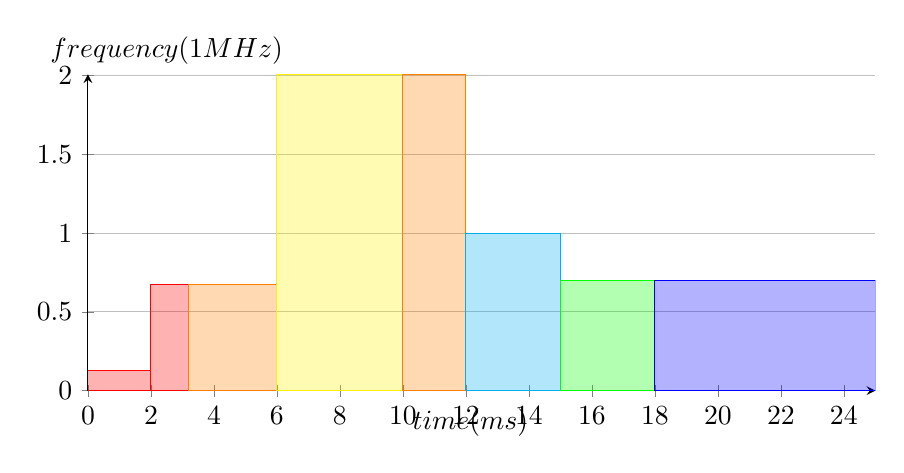
\begin{tikzpicture}
      \begin{axis}[x=0.4cm, y=2cm, xtick={0, 2, ..., 25}, ytick={0, 0.5, ...,2}, axis lines=left,
        ymajorgrids=true, ymin=0, xlabel=$time (ms)$, xlabel style={at={(0.4,-0.1)}, anchor=west},
        ylabel=$frequency (1 MHz)$, ylabel style={rotate=-90,at={(0.1,1)}, anchor=south}
        ]
      \addplot [
        ybar interval,
        xtick=data,
        x tick label style={
        rotate=90,
        anchor=east,
        },
        color=red, fill=red, fill opacity=0.3
      ] coordinates {
        (0,0.125) (2,0.675) (3.2,0.675)
      };
      \addplot [
        ybar interval,
        xtick=data,
        x tick label style={
        rotate=90,
        anchor=east,
        },
        color=orange, fill=orange, fill opacity=0.3
      ] coordinates {
        (3.2,0.675) (6,0.675)
      };
      \addplot [
        ybar interval,
        xtick=data,
        x tick label style={
        rotate=90,
        anchor=east,
        },
        color=yellow, fill=yellow, fill opacity=0.3
      ] coordinates {
        (6,2.0083) (9.983,2.0083)
      };
      \addplot [
        ybar interval,
        xtick=data,
        x tick label style={
        rotate=90,
        anchor=east,
        },
        color=orange, fill=orange, fill opacity=0.3
      ] coordinates {
        (9.983,2.0083) (12,2.0083)
      };
      \addplot [
        ybar interval,
        xtick=data,
        x tick label style={
        rotate=90,
        anchor=east,
        },
        color=cyan, fill=cyan, fill opacity=0.3
      ] coordinates {
        (12,1) (15,1)
      };
      \addplot [
        ybar interval,
        xtick=data,
        x tick label style={
        rotate=90,
        anchor=east,
        },
        color=green, fill=green, fill opacity=0.3
      ] coordinates {
        (15,0.7) (18,0.7)
      };
      \addplot [
        ybar interval,
        xtick=data,
        x tick label style={
        rotate=90,
        anchor=east,
        },
        color=blue, fill=blue, fill opacity=0.3
      ] coordinates {
        (18,0.7) (25,0.7)
      };
    \end{axis}
    \end{tikzpicture}
  \end{solutionnoinc}
\end{frame}
